% #############################################################################
% This is Chapter 4
% !TEX root = ../main.tex
% #############################################################################
% Change the Name of the Chapter i the following line
\fancychapter{Algorithmic Optimization in Architecture}
\cleardoublepage
% The following line allows to ref this chapter
\label{chap:implement}

In the last chapter, we discussed the architecture of the proposed solution, a general purpose optimization framework that is applicable to solve any optimization problem. 

From the beginning, we set out to address optimization problems involving costly evaluation functions that may take up to several minutes, hours, or even days to complete. Therefore, during the development of the proposed framework, we focused on problems exhibiting these properties. Note, however, that the framework can be easily extended to include other algorithms (e.g., derivative-based), as it has been previously discussed in \Cref{sec:optalgos}. 

Motivated by the large impact of the building sector in the world's sustainability and economy, this dissertation aims at applying the proposed framework to address building design optimization, thus attempting to reduce buildings' costs and ecological footprint. Despite the existence of multiple optimization tools in architecture (see~\Cref{sec:plugins}), these are often limited and do not provide adequate algorithms, nor mechanisms to enable the efficient optimization of problems with time-consuming evaluations (see~\Cref{sec:problemsaddress}).

In this chapter, we describe how the general-purpose framework proposed in this dissertation can be applied to address architectural design optimization. 

\section{Algorithmic Optimization}

In \Cref{ssec:ad,ssec:aa}, we discussed how architectural paradigms have incrementally grown to develop the mechanisms to quickly (1) update a design, (2) generate the corresponding analytical model, and (3) automatically evaluate the design in an analytical tool and collect its results. 

These mechanisms laid down the foundations for automated optimization processes. By extending the Algorithmic Design (AD) and Algorithmic Analysis (AA) approaches to include optimization mechanisms, we are able to apply automatic optimization processes that aim to improve (or even optimize) designs' performance. 

\Cref{fig:algorithmicoptimization} illustrates a possible approach for introducing automated optimization processes in the architectural worfklow. In this approach, we introduce an optimizer component that is responsible for searching the design space and generating new values for the design's parameters. These values are then communicated to the \ac{AD} tool, which generates the corresponding analytical models and evaluates them in the corresponding analytical tools. After being evaluated, the analytical tools communicate the evaluations' results to the \ac{AD} tool, which, in turn, forwards them to the optimizer. Based on these results, the optimizer generates other set of values for the design's parameters and this process is repeated until a stopping criterium (e.g., evaluations or time limit, solution's quality) is met. The communications between each component are encoded within the \ac{AD} tool, therefore incurring no additional efforts for the programmer.
 
 \begin{figure}[htbp]
 	\centering
 	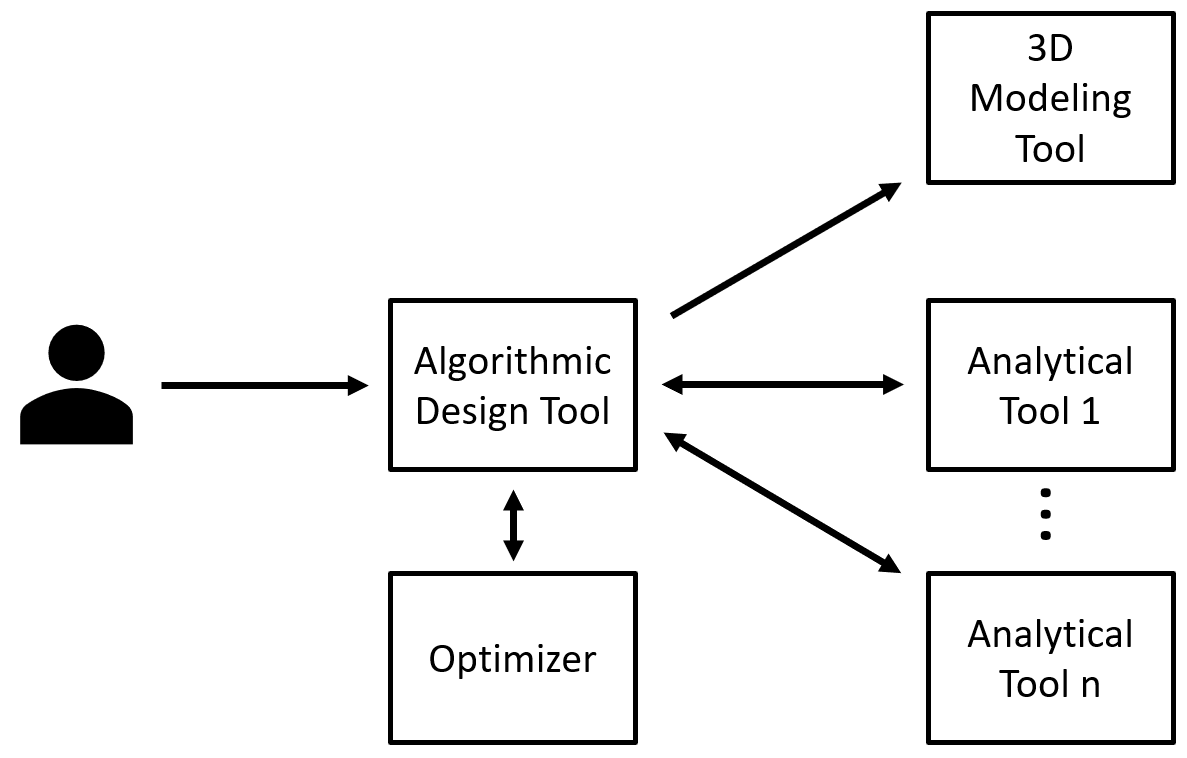
\includegraphics[width=0.6\textwidth]{./Images/Solution/algorithmic_optimization.png}
 	\caption{Algorithmic Optimization workflow. In this workflow, the user only interacts with an \ac{AD} tool to create the initial design, to specify the analysis tools, and to specify the optimization parameters.}
 	\label{fig:algorithmicoptimization}
 \end{figure}
 
In order to benefit from the \ac{AO} approach, we combine the optimization framework developed in this dissertation with an \ac{AD} tool to provide an alternative easily address a wide variety of \ac{BPO} problems. To this end, architects are required to: (1) create the \ac{AD} model reflecting their design's intents; (2) select the performance aspects to optimize and, thus, the analysis tools to be used (e.g., lighting, thermal, structural, costs), and, finally, (3) to select, if necessary, the parameters of the optimization process (e.g., algorithm, algorithm's parameters). In the end, architects are only required to run the script and the optimization process will automatically start. \Cref{BPOjuliaCode} presents a simple example of an \ac{AO} approach using the developed framework and the \ac{AD} Khepri tool, where the architect: (1) defines the algorithmic description of the intended design (\textit{lines 1-3}), (2) defines four variables and their acceptable variation range (\textit{lines 20-23}), (3) define the objective functions for the performance aspects to consider in the optimization (\textit{lines 6-17 and 24-25}), (4) creates the optimization model (\textit{line 26}), (5) defines the algorithm's parameters (\textit{line 27}), and (6) specifies the optimization algorithm and the maximum number of evaluations (\textit{line 28}).

Even though the provided example presents a textual-based \ac{AO} approach, the developed optimization framework can easily be integrated within a visual \ac{AD} tool, like Grasshopper. 

An important aspect that the results of this combination is the fact that architects are able to use different optimization algorithms and, consequently, to select an optimization algorithm that better suits their problems. To bridge the gap between the lack of knowledge or experience and the suitability of optimization algorithms for each problem, the optimization framework also provides automated testing mechanisms. These mechanisms enable the sequential execution of multiple optimization algorithms for a specified amount of evaluations, as well as each algorithm's performance measures. This feature is particularly important in the architectural context~\cite{Wortmann2016BBO,Hamdy2016}, as it promotes more informed decisions towards the selection of more appropriate optimization algorithms.


\begin{lstlisting}[caption={BPO example of the framework's API using the Khepri AD tool.},label=BPOjuliaCode]	
building_with_skylight(height, width, length, material) = let
	# Create the design using Khepri's primitives
	...
end

# Analytical-based criterium
cost_performance(height, width, length, material) = let
	p1 = scale(width, 1.5) * scale(length, 6.5) * 185
	p2 = (scale(width, 1.5) + scale(length, 6.5)) * 2 * height * 80
	p1 + p2
end

# Simulation-based criterium
daylight_performance(height, width, length, material) = radiance_analysis(
	() -> building_with_skylight(height, width, length, material)) do results
		...
end

# Optimization Process
let height = RealVariable(0.1, 2),
	width = RealVariable(0.1, 6.5),
	length = RealVariable(0.1, 11),
	material = IntVariable(0, 3),
	obj1 = Objective(daylight_performance, :MAX),
	obj2 = Objective(cost_performance, :MIN),
	model = Model([height, width, length, material], [obj1, obj2]),
	NSGA_params = Dict(:population_size => 10)
  solve(NSGAII, NSGA_params, model, max_evals=100)
end
\end{lstlisting}


Another key aspect of this framework is the ability to post-process and visualize the data resulting from the optimization process. On the one hand, a good representation enables architects to detect errors or incoherences (e.g., with the optimization model) early in the optimization process. Besides errors, it also fosters less time-consuming optimization processes for interactive and real-time scenarios, where these representations are updated with the new information that results from the optimization. In such scenarios, architects are able to explore the different evaluated candidate solutions and identify whether any of the already evaluated solutions is good enough for the specified problem, even if it is not an optimum.

On the other hand, a good data representation also enhances the comprehension of the optimization process itself. By providing automatic visual representations the optimization results, architects are able to reason and to create logical patterns that allow them to explain the obtained results. As a result, besides getting a more clear perspective about the optimization process, architects are also able to learn more about their designs' behavior for different performance aspects and, potentially, about the optimization algorithm itself.
